%%%%%%%%%%%%%%%%%%%%%%%%%%%%%%%%%%%%%%%%%%%%%%%%%%%%%%%%%%%%%%%%%%%%%%%%%%%%%%%%%%%%%%%%%%%%%%%%%%%%%%%%%%%%%%%
%% Modelo de tese com capítulos individuais
%% 
%% Neste formato, cada capítulo é preparado de maneira que possa ser lido individualmente, muitas vezes baseado
%% em trabalho publicado em revista científica na forma de artigo. Assim sendo, cada capítulo possui 
%% aproximadamente a mesma estrutura de um artigo, quais sejam: resumo, abstract, introdução, material e 
%% métodos, resultados, discussão, e conclusões.
%%%%%%%%%%%%%%%%%%%%%%%%%%%%%%%%%%%%%%%%%%%%%%%%%%%%%%%%%%%%%%%%%%%%%%%%%%%%%%%%%%%%%%%%%%%%%%%%%%%%%%%%%%%%%%%

%%=============================================================================================================
%% Definições gerais - tipo de documento
%%=============================================================================================================

%% Tipo de documento e a classe a ser usada para sua formatação.
\documentclass[tese, header, newmargins]{UFRuralRJ}

%% A opção 'openright' força inícios de capítulos em páginas ímpares
%\documentclass[openright]{UFRuralRJ}

%% Use a opção 'twoside' para gerar uma versão frente-e-verso
%\documentclass[twoside]{UFRuralRJ}

%%=============================================================================================================
%% Pacotes - língua, codificação e fonte
%%=============================================================================================================
\usepackage[brazilian]{babel} %% use 'english' para documento escrito em inglês
\usepackage[T1]{fontenc} %% Conjunto de caracteres correto
\usepackage[utf8]{inputenc} %% Para acentuação correta

%%=============================================================================================================
%% Pacotes - formatação de equações e números
%%=============================================================================================================

\usepackage{amsmath,latexsym,amssymb}
\usepackage{siunitx} %% Sistema Internacional de Unidades

%%=============================================================================================================
%% Pacotes - formatação de figuras
%%=============================================================================================================

%% Importar figuras corretamente
\usepackage{graphicx}

%% Diretório onde estão as figuras dos capítulos
\graphicspath{{capitulos-b/figuras/}}

\usepackage{float}
\usepackage{wrapfig}

%%=============================================================================================================
%% Pacotes - formatação de hyperlinks e urls
%%=============================================================================================================

%% Opção 'hidelinks' disponível no pacote 'hyperref' a partir da versão 2011-02-05  6.82a. 'hidelinks' retira 
%% os retângulos do entorno das palavras com links.

\usepackage[%hidelinks%, 
            bookmarksopen=true, linktoc=page, colorlinks=true,
            linkcolor=blue, citecolor=blue, filecolor=magenta, urlcolor=blue,
            pdftitle={UFRuralRJ -- Classe LaTeX para formatação de documentos acadêmicos na UFRRJ},
            pdfauthor={Graziela Barroso},
            pdfsubject={Tese de Doutorado},
            pdfkeywords={LaTeX, UFRuralRJ, Documentos acadêmicos}
            ]{hyperref}

%% Pacote para lidar com url longa, deve ser carregado depois do pacote 'hyperref'
\usepackage[hyphenbreaks]{breakurl}

%% Se o pacote 'hyperref' acima foi carregado, a linha abaixo corrige um bug na 
%% hora de montar o sumário da lista de figuras e tabelas. Comente a linha se o
%% pacote 'hyperref' não foi carregado.

%%=============================================================================
%% Trampa para corrigir o bug do hyperref que redefine o caption das figuras e das
%% tabelas, n�o colocando o nome ``Figura'' antes do n�mero do mesmo na lista
%%=============================================================================

\makeatletter

\long\def\@caption#1[#2]#3{%
  \expandafter\ifx\csname if@capstart\expandafter\endcsname
                  \csname iftrue\endcsname
    \global\let\@currentHref\hc@currentHref
  \else
    \hyper@makecurrent{\@captype}%
  \fi
  \@ifundefined{NR@gettitle}{%
    \def\@currentlabelname{#2}%
  }{%
    \NR@gettitle{#2}%
  }%
  \par\addcontentsline{\csname ext@#1\endcsname}{#1}{%
    \protect\numberline{\csname fnum@#1\endcsname ~-- }{\ignorespaces #2}%
  }%
  \begingroup
    \@parboxrestore
    \if@minipage
      \@setminipage
    \fi
    \normalsize
    \expandafter\ifx\csname if@capstart\expandafter\endcsname
                    \csname iftrue\endcsname
      \global\@capstartfalse
      \@makecaption{\csname fnum@#1\endcsname}{\ignorespaces#3}%
    \else
      \@makecaption{\csname fnum@#1\endcsname}{%
        \ignorespaces
        \ifHy@nesting
          \expandafter\hyper@@anchor\expandafter{\@currentHref}{#3}%
        \else
          \Hy@raisedlink{%
            \expandafter\hyper@@anchor\expandafter{%
              \@currentHref
            }{\relax}%
          }%
          #3%
        \fi
      }%
    \fi
    \par
  \endgroup
}

\makeatother

%%=============================================================================================================
%% Pacotes - formatação da bibliografia de acordo com as normas da ABNT
%%=============================================================================================================
% O pacote 'abntex2cite' precisa, obrigatoriamente, ser carregado depois do pacote 'hyperref'.
% Mais informações podem ser obtidas na página do pacote no GitHub: https://github.com/abntex/abntex2

\usepackage[alf, abnt-and-type=&, abnt-etal-cite=2, abnt-etal-list = 0]{abntex2cite}

%%=============================================================================================================
%% Pacotes - formatação de verbatim
%%=============================================================================================================
%% O ambiente verbatim é o ambiente onde são inseridos exemplos de código fonte.
%% Está opção adiciona cor de fundo ao ambiente verbatim.
%% Comente para desabilitar.

\let\oldv\verbatim
\let\oldendv\endverbatim
\def\verbatim{\par\setbox0\vbox\bgroup\oldv}
\def\endverbatim{\oldendv\egroup\fboxsep0pt 
                 \noindent\colorbox[gray]{0.8}{\usebox0}\par}

%%=============================================================================================================
%% Pacotes - outros
%%=============================================================================================================

% \usepackage{showframe}

\usepackage{blindtext} %% Amostra de texto (\blindtext[1])

%%=============================================================================================================
%% Identificação do trabalho
%%=============================================================================================================
\titulo{UFRuralRJ -- Classe \LaTeX{} para Formatação de Documentos Acadêmicos na UFRRJ} %% Título
\author{Barroso}{Graziela} %% Autor: sobrenome, nome
\autoratrue %% Usar no caso de uma AUTORA
\instituto{Instituto de Agronomia} %% Instituto
\curso{Curso de Pós-Graduação em Agronomia -- Ciência do Solo} %% Curso de pós-graduação
\area{Ciência do Solo} %% Área de concentração
\local{Seropédica}{RJ}{Brasil} %% Local da defesa

%%=============================================================================================================
%% Identificação dos orientadores
%%=============================================================================================================
\advisor[Professora]{Dra.}{Dobereimer}{Johana}{UFRRJ} %% Orientadora
\coadvisor[Pesquisador]{Dr.}{Salles}{Hilton} %% Co-orientador
\coadvisor[Professor]{Dr.}{Costa}{Fernando} %% Co-orientador

%%=============================================================================================================
%% Informações sobre a defesa
%%=============================================================================================================
\committee[Dr.]{Raithe}{Waldemar}{UFRRJ} %% Presidente
\committee[Dra.]{Campos}{Maria Aparecida}{UFRRJ} %% Examinadora
\committee[Dr.]{Peçanha}{Gilberto Gastim}{UFRRJ} %% Examinador
\committee[Dra.]{Souza}{Tânia Maria Melquiades de}{UFRRJ} %% Examinadora
\committee[Dr.]{Groszman}{Américo}{UFRRJ} %% Examinador
\date{30}{Fevereiro}{2001} %% Data da defesa

%%=============================================================================================================
%% Início do documento
%%=============================================================================================================
\begin{document}

%%=============================================================================================================
%% Capa e folha de rosto
%%=============================================================================================================
\maketitle

%%=============================================================================================================
% Folha de aprovação
%%=============================================================================================================
\makeapprove

%%=============================================================================================================
%% Dedicatória (opcional)
%%
%% NOTA: Usar versão estrelada de 'chapter'
%%=============================================================================================================
\chapter*{}
\vfill
\begin{flushright}
  {\em
  Àqueles que financiaram meu trabalho...
  \par
  ...DEDICO!
  }
\end{flushright}

%%=============================================================================================================
%% Agradecimentos (opcional)
%%
%% NOTA: Usar versão estrelada de 'chapter'
%%=============================================================================================================
\chapter*{Agradecimentos}

\noindent{À Universidade Federal Rural do Rio de Janeiro.}

\noindent{Às agências de fomento.}

\noindent{Aos orientadores.}

\noindent{À todos que, direta ou indiretamente, contribuíram para a construção deste trabalho.}

%%=============================================================================================================
%% Biografia (opcional)
%%
%% NOTA: Usar versão estrelada de 'chapter'
%%=============================================================================================================
\chapter*{Biografia}
\noindent{O autor nasceu, cresceu e escreveu uma tese.}

%%=============================================================================================================
%% Epígrafe (opcional)
%%
%% NOTA: Usar versão estrelada de 'chapter'
%%=============================================================================================================
\chapter*{}
\vfill
\begin{flushright}
  {\em
  ``Fazer é a melhor forma de dizer.''
  \par
  Autor desconhecido
  }
\end{flushright}

%%=============================================================================================================
%% Resumo geral (português)
%%=============================================================================================================
\def\tituloPT{UFRuralRJ -- Classe \LaTeX{} para formatação de documentos acadêmicos na UFRRJ}
\def\chavesPT{\LaTeX. UFRuralRJ. Documentos acadêmicos} %% Palavras-chave em português
\def\nivelPT{Doutorado em Agronomia, Ciência do Solo} %% Nível do curso ou grau obtido em português

\generalabstracttrue %% Usar para o caso de um RESUMO GERAL
\begin{generalabstract}{brazilian}{\tituloPT}{\chavesPT}{\nivelPT} %% Resumo geral em português
Este é o resumo geral em português de minha tese organizada na forma de capítulos individuais. Claramente, 
este é o melhor resumo que já foi escrito em um documento acadêmico produzido na UFRuralRJ.
\end{generalabstract}

%%=============================================================================================================
%% General abstract (inglês)
%%=============================================================================================================
\def\tituloEN{UFRuralRJ -- \LaTeX{} class for formatting academic documents at UFRRJ}
\def\chavesEN{\LaTeX. UFRuralRJ. Academical documents} %% Palavras-chave em inglês
\def\nivelEN{Doctor of Science in Agronomy, Soil Science} %% Nível do curso ou grau obtido em inglês

\generalabstracttrue
\begin{generalabstract}{english}{\tituloEN}{\chavesEN}{\nivelEN} %% Resumo geral em inglês
This is the English abstract of my thesis organized in the form of individual chapters. Obviously this is the 
best abstract that has ever been written in an academic document produced at UFRuralRJ.
\end{generalabstract}

%%=============================================================================================================
%% Listas (comentar se não houver) e sumário
%%=============================================================================================================

\listoffigures %% Lista de figuras
% \listoftables %% Lista de tabelas
\listofappendix %% Lista de apêndices
% \listofannex %% Lista de anexos

\begin{listofabbrv}{UbiComp} %% Lista de abreviaturas e siglas
 \item [RJ] Rio de Janeiro
 \item [UFRuralRJ] Universidade Federal Rural do Rio de Janeiro
\end{listofabbrv}

\begin{listofsymbols}{teste} %% Lista de simbolos
 \item [$\varnothing$] vazio %% Simbolos devem aparecer conforme a ordem em que aparecem no texto
 \item [$\Gamma$]  Gama      %% O parâmetro deve ser o símbolo mais longo
 \item [$\forall$] Para todo
\end{listofsymbols}

\tableofcontents %% Sumário

%%=============================================================================================================
%% Início da tese
%%=============================================================================================================

\setcounter{page}{1}
\artigofalse
\chapter{Introdução}
\label{chap:introduction}

\blindtext[2]

\begin{figure}[!ht]
\centering
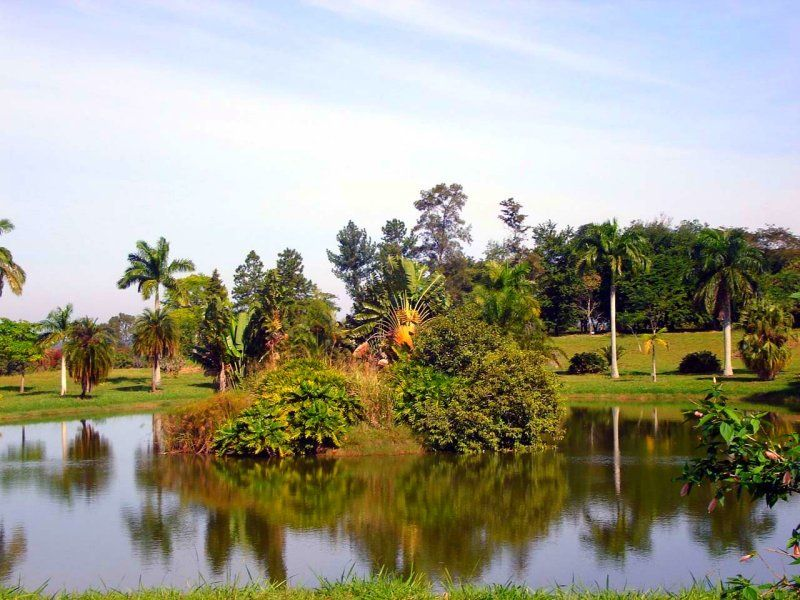
\includegraphics[width=16cm]{figura01}
\caption{Jardim Botânico da UFRuralRJ. Fonte: \url{http://commons.wikimedia.org/wiki/File:Jardim_Bot\%C3\%A2nico_UFRRJ.jpg}}
\label{fig:jardim}
\end{figure}

\blindtext[1]

\section{SEÇÃO}

\blindtext[2]

\subsection{Subseção}

\blindtext[2] %% Incluir Introdução Geral
\artigotrue
\chapter{Título do Primeiro artigo}
\label{chap:chapter01}

\begin{chapterabstract}{brazilian}{Palavra-chave 1, Palavra-chave 2, Palavra-chave 3}
Este é o resumo do primeiro artigo da tese.
\end{chapterabstract}

\begin{chapterabstract}{english}{Key-word 1, Key-word 2, Key-word 3}
This is the abstract of the first article of the thesis.
\end{chapterabstract}

\formatchapter

\section{Introdução}

\blindtext[2]

\section{Material e métodos}

Este é um texto bem formatado, escrito em Seropédica, RJ. \blindtext[1]

Este é o código fote de uma função construída no ambiente R:

\begin{verbatim}
> soma <- function (a, b) {a + b}
> soma(2, 2)
[1] 4
\end{verbatim}

Está é uma matriz bem formatada:

\begin{equation}
  A_{m,n} =
 \begin{pmatrix}
  a_{1,1} & a_{1,2} & \cdots & a_{1,n} \\
  a_{2,1} & a_{2,2} & \cdots & a_{2,n} \\
  \vdots  & \vdots  & \ddots & \vdots  \\
  a_{m,1} & a_{m,2} & \cdots & a_{m,n}
 \end{pmatrix}
\end{equation}

\begin{subequations}\label{eq:maxwell}
E estas são as equações de Maxwell:
\begin{align}
        B'&=-\nabla \times E,\\
        E'&=\nabla \times B - 4\pi j,
\end{align}
\end{subequations}

\section{Resultados}

Aqui está mais um texto bem formatado. \blindtext[1]

Que tal fazer um link para a figura \autoref{fig:ocio}? E também citar o \citet{Feyerabend1977} com um link para a localização da referência bibliográfica?

\begin{figure}[!ht]
\centering
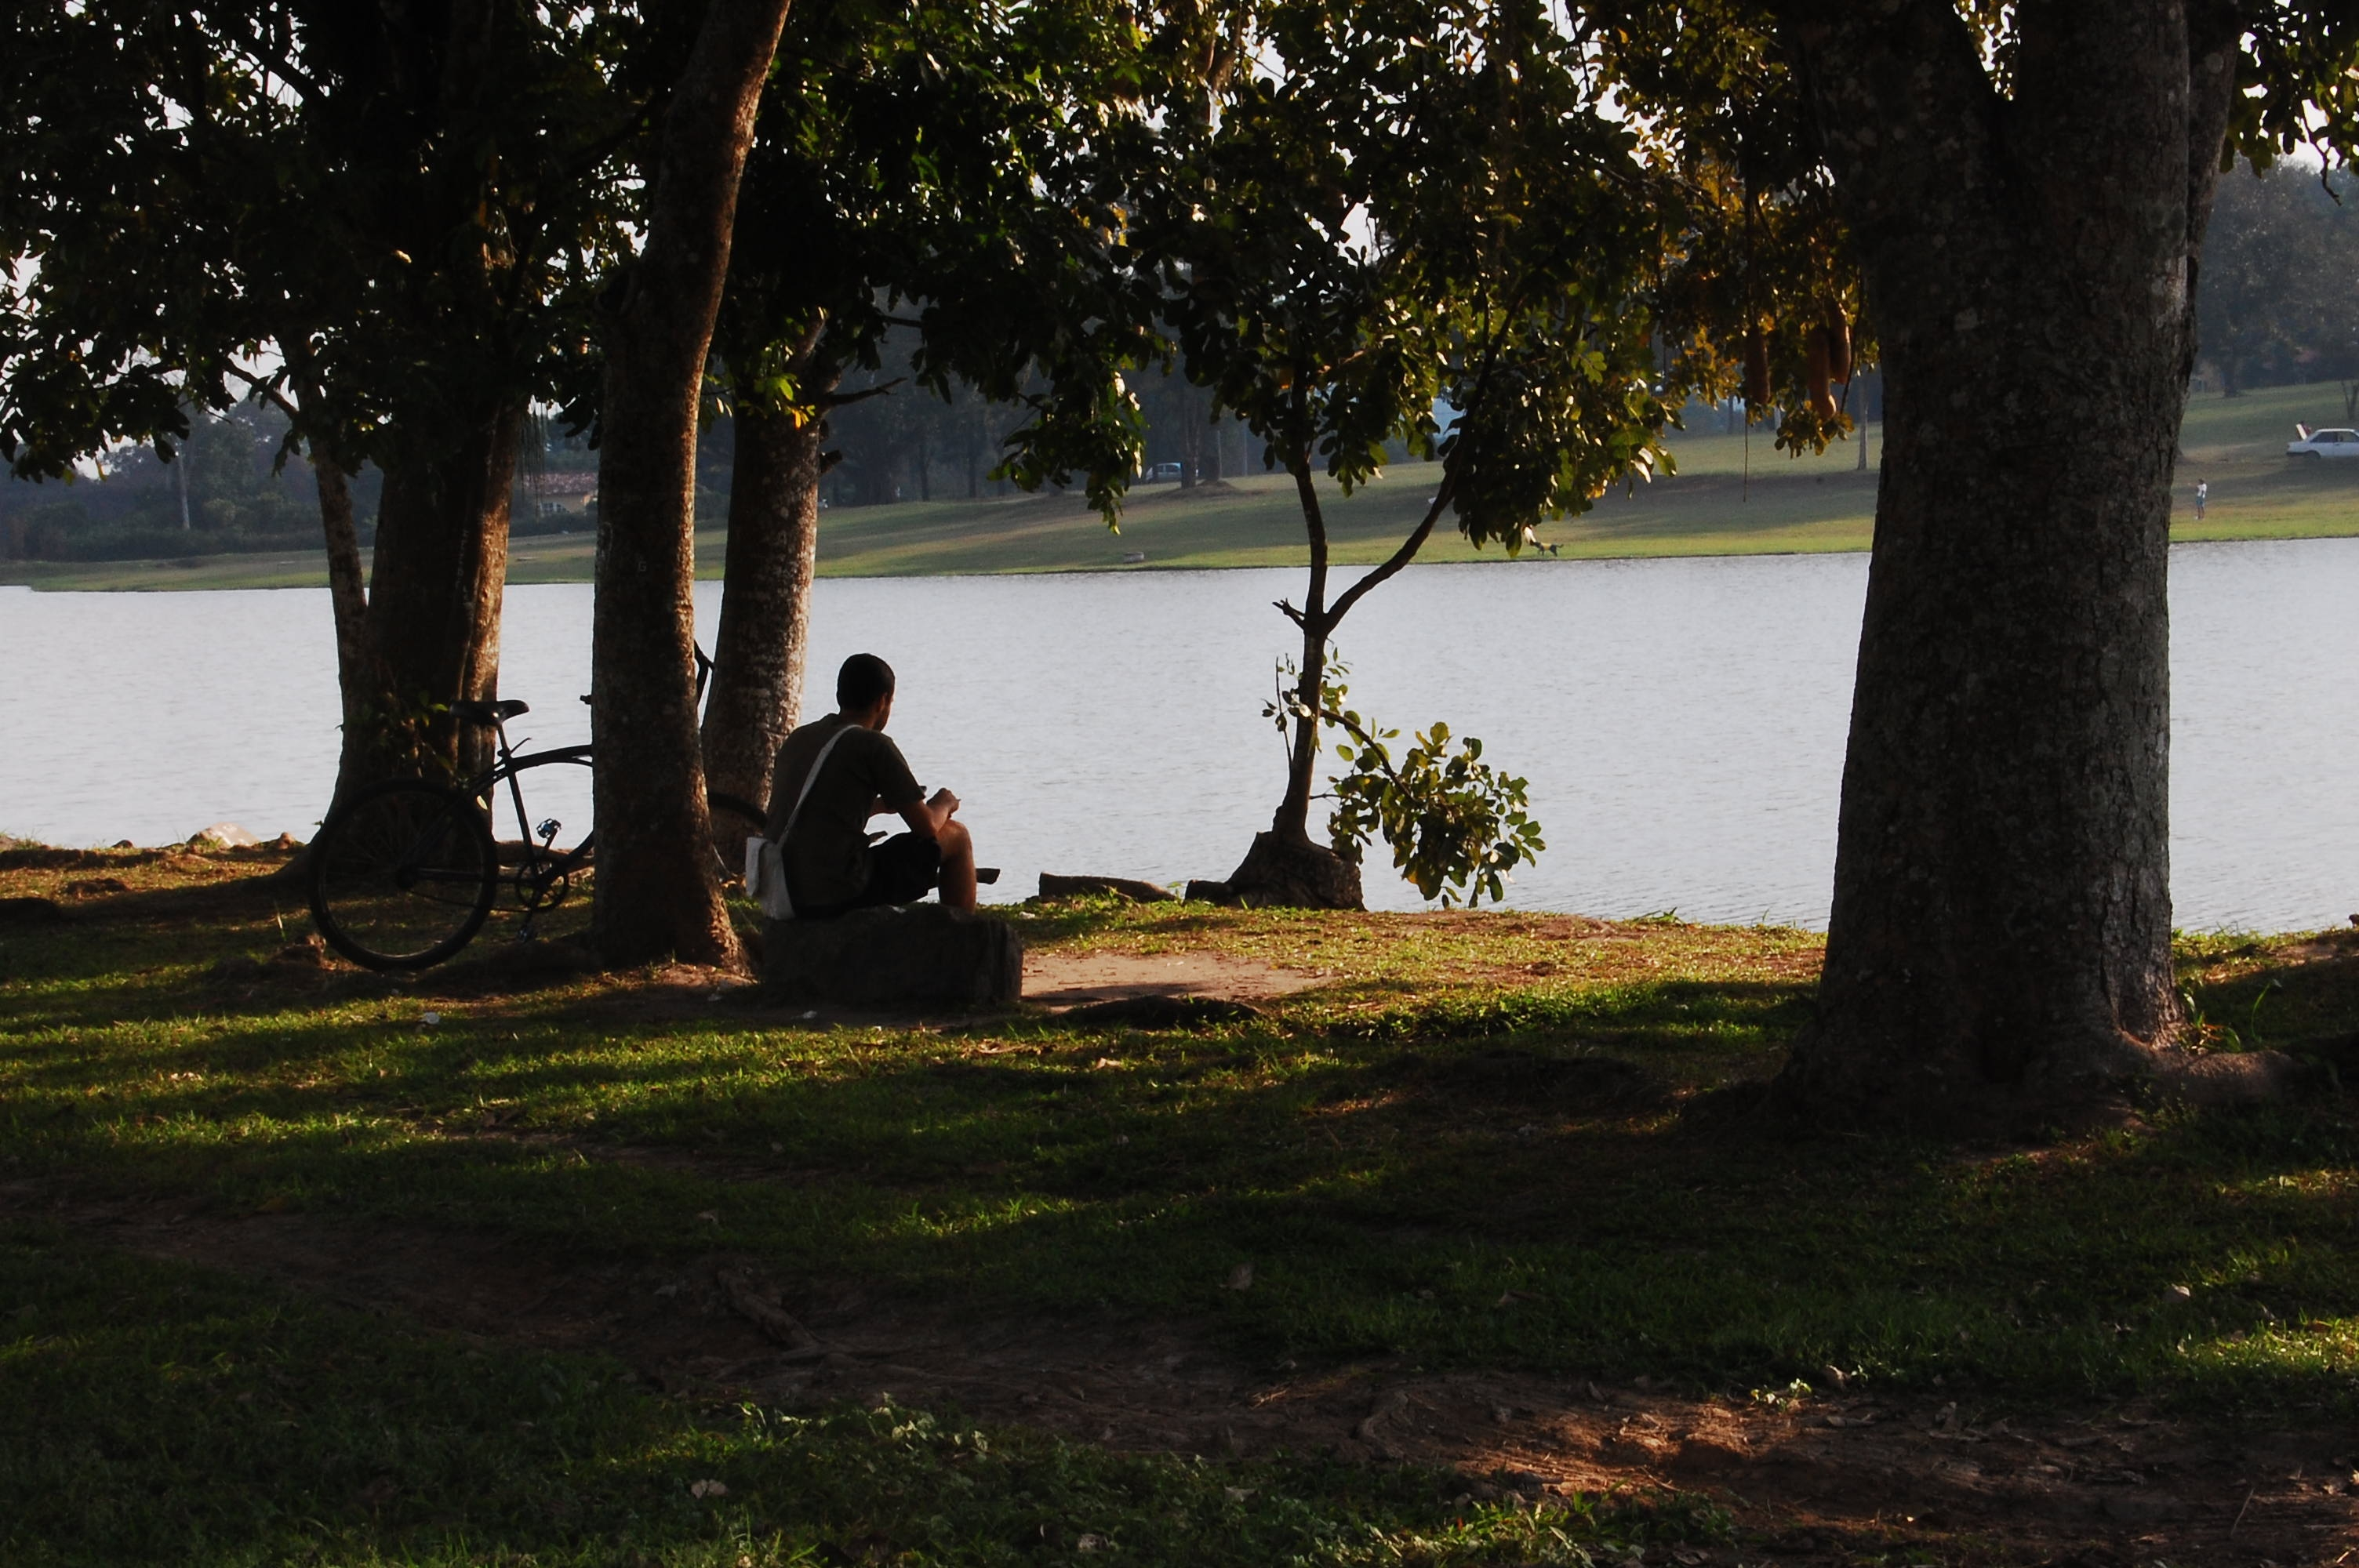
\includegraphics[width=16cm]{figura02}
\caption{\label{fig:ocio}O ócio criativo. Fonte: \url{http://r1.ufrrj.br/graduacao/img/acesso-2012/o-ocio-criativo.jpg}}
\end{figure}

\section{Discussão}

Aqui está o último texto muito bem formatado. \blindtext[2]

Que tal fazer um link para a equação \autoref{eq:maxwell}?

\section{Conclusões}

\begin{itemize}
  \item Está é uma conclusão importante.
  \item Está é outra conclusão importante.
  \item Está é uma conclusão menos importante.
\end{itemize}
 %% Incluir capítulo 01
\artigotrue
\chapter{TÍTULO DO SEGUNDO ARTIGO}
\chapternote{Este capítulo é baseado em um artigo que já foi publicado.}
\shorttitle{Segundo artigo}
\label{chap:chapter01}

\begin{chapterabstract}{brazilian}{Palavra-chave 1. Palavra-chave 2. Palavra-chave 3}
Este é o resumo do segundo artigo da tese. Reconheço que este artigo não é muito
diferente do anterior... Mas quem se importa?
\end{chapterabstract}

\begin{chapterabstract}{english}{Key-word 1. Key-word 2. Key-word 3}
This is the abstract of the second article of the thesis. I recognize that it is
not very different from the previous... But who cares?
\end{chapterabstract}

\formatchapter

\section{INTRODUÇÃO}

\blindtext[2]

\section{MATERIAL E MÉTODOS}

Este também é um texto bem formatado, escrito em Seropédica, RJ. \blindtext[1]

Este é o código fonte de uma função muito complexa construída no ambiente R:

\begin{verbatim}
> soma <- function (a, b) {a + b}
> soma(2, 2)
[1] 4
\end{verbatim}

Está é uma matriz bem formatada, diferente daquelas produzidas pelos editores de
texto tradicionais:

\begin{equation}
  A_{m,n} =
 \begin{pmatrix}
  a_{1,1} & a_{1,2} & \cdots & a_{1,n} \\
  a_{2,1} & a_{2,2} & \cdots & a_{2,n} \\
  \vdots  & \vdots  & \ddots & \vdots  \\
  a_{m,1} & a_{m,2} & \cdots & a_{m,n}
 \end{pmatrix}
\end{equation}

\begin{subequations}\label{eq:maxwell2}
E estas são as equações de Maxwell (sim, de Maxwell!):
\begin{align}
        B'&=-\nabla \times E,\\
        E'&=\nabla \times B - 4\pi j,
\end{align}
\end{subequations}

\section{RESULTADOS}

Para quem ainda não está cansado, aqui está mais um texto bem formatado. 
\blindtext[1]

Que tal fazer um link para a \autoref{fig:ocio2}? E também citar o 
\citeonline{Feyerabend1977} com um link para a localização da referência 
bibliográfica? Sim, isso já foi feito antes!

\begin{figure}[!ht]
\label{fig:ocio2}
\centering
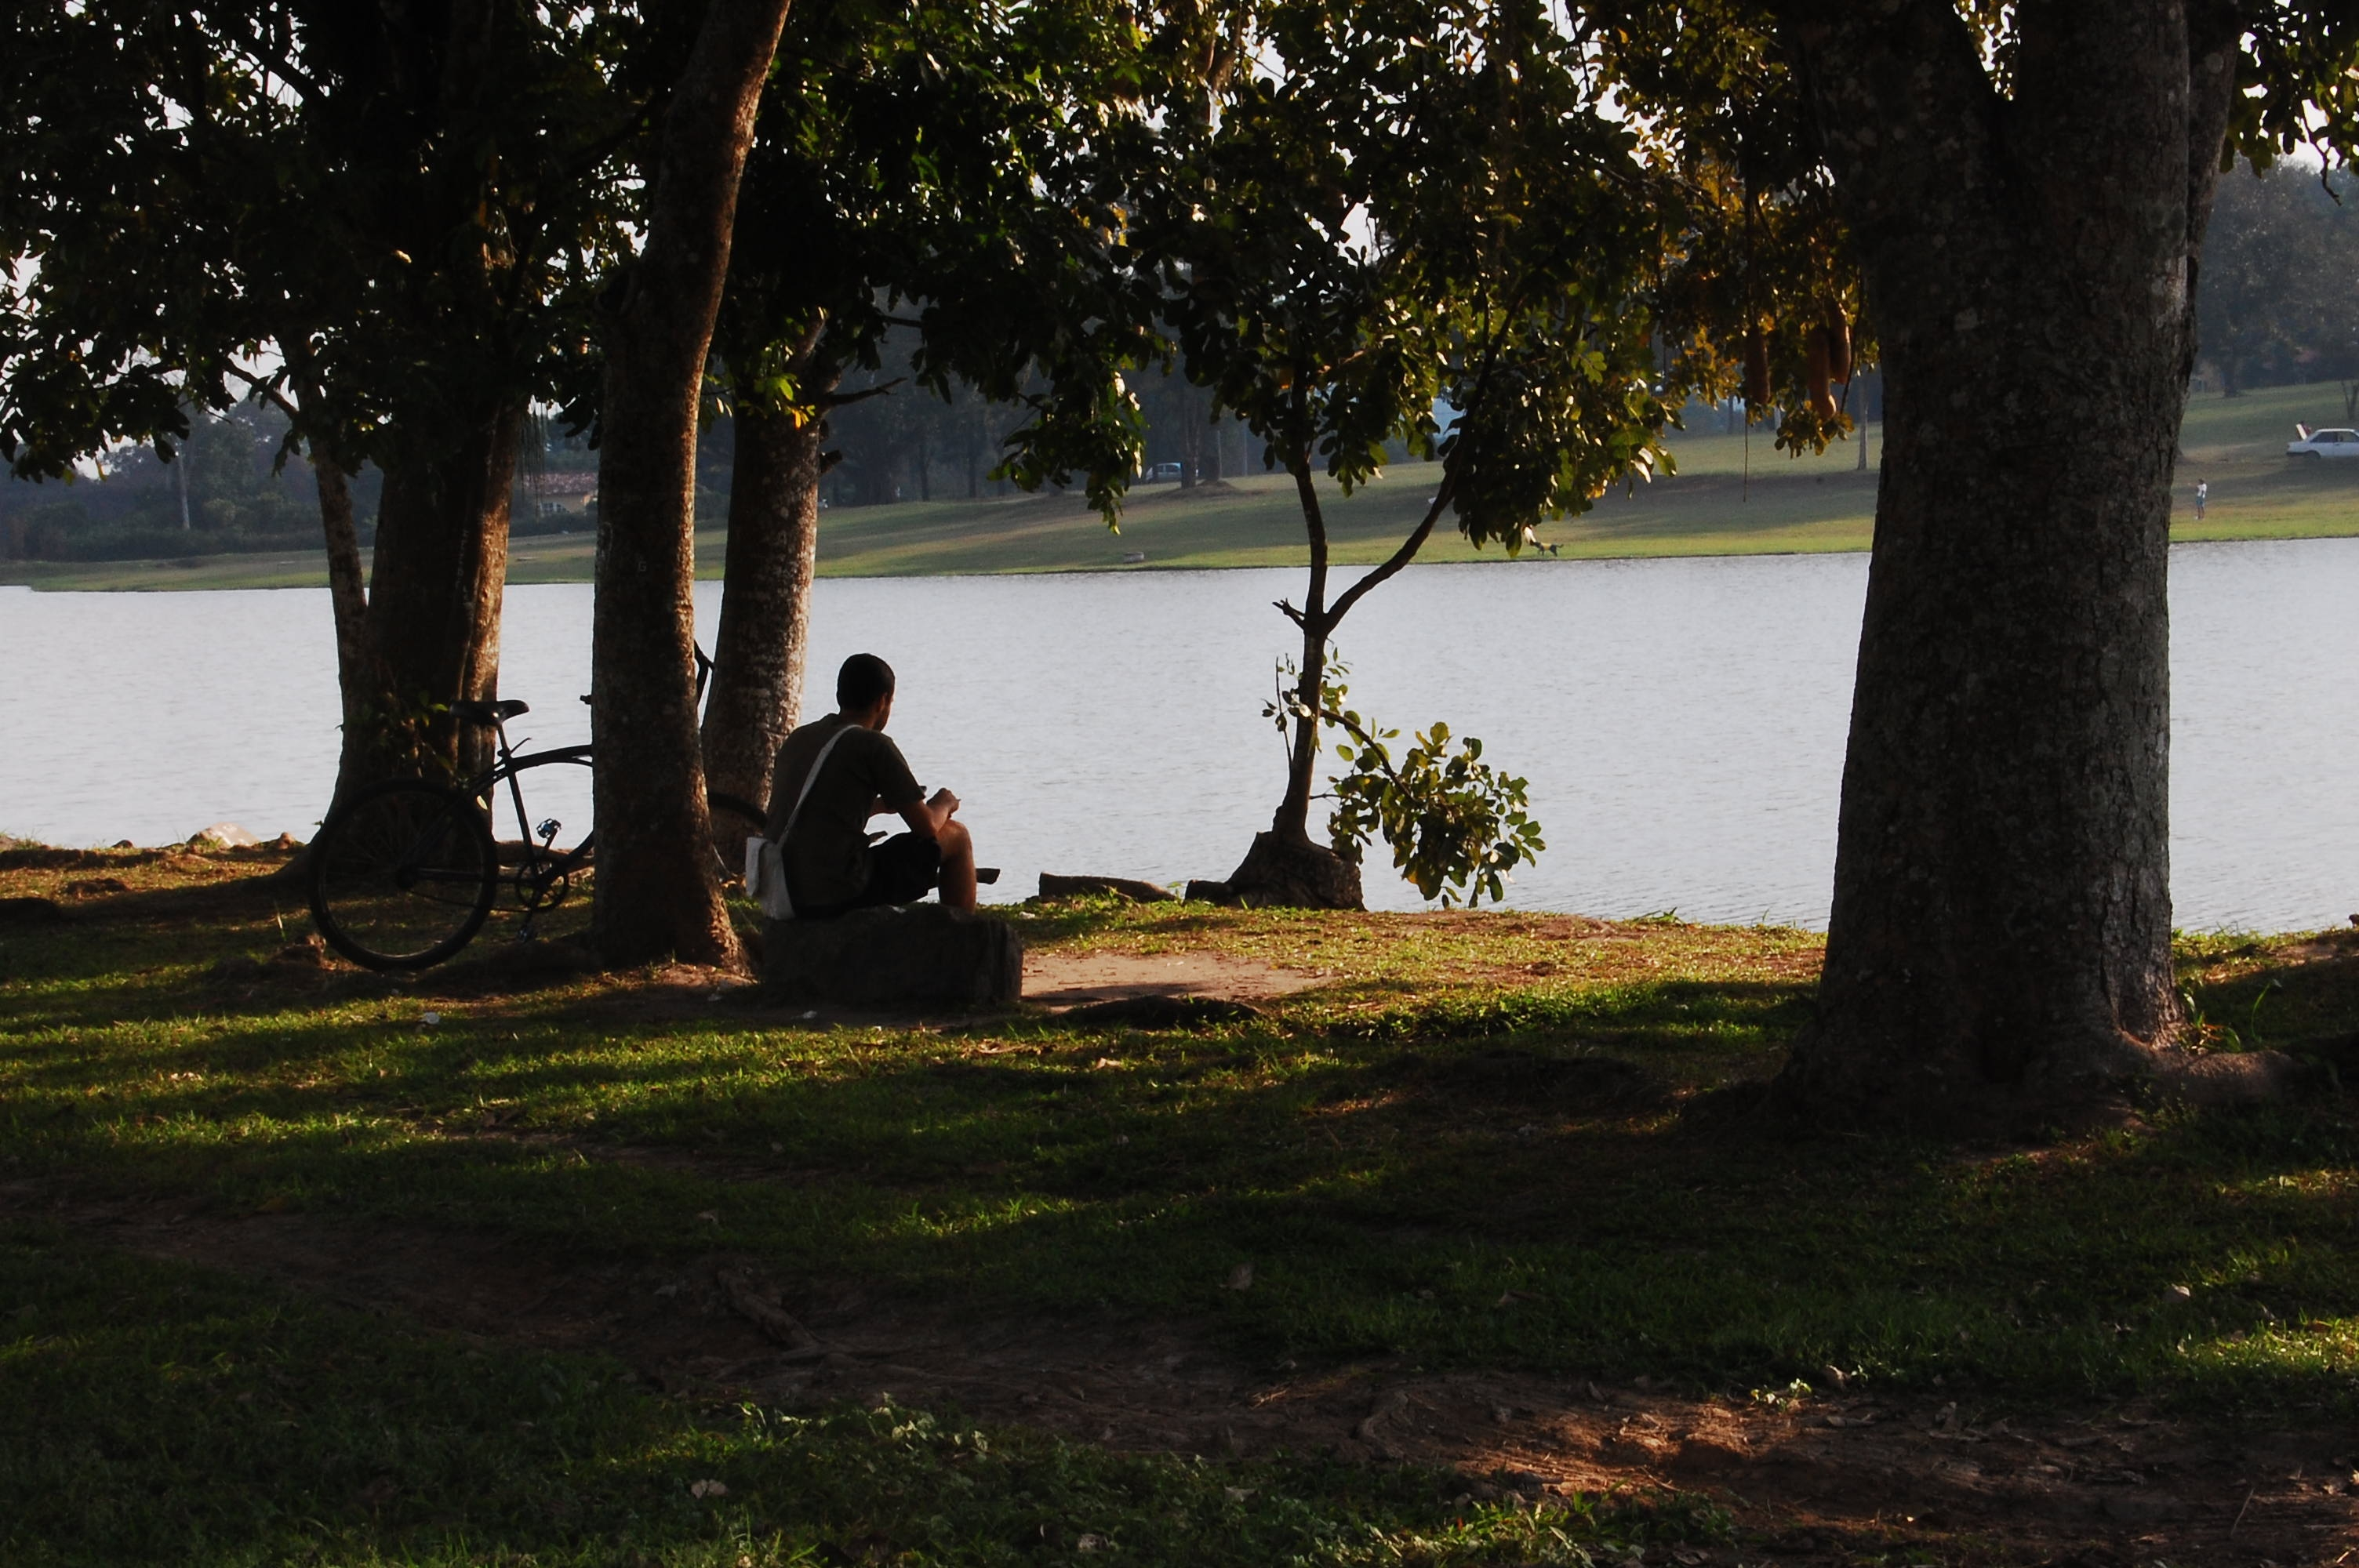
\includegraphics[width=16cm]{figura02}
\caption[O ócio criativo.]{O ócio criativo. Fonte: 
\url{http://r1.ufrrj.br/graduacao/img/acesso-2012/o-ocio-criativo.jpg}}
\end{figure}

\section{DISCUSSÃO}

Aqui está o último texto muito bem formatado. \blindtext[2]

Que tal fazer um link para a \autoref{eq:maxwell2}?

\section{CONCLUSÕES}

\begin{itemize}
  \item Está é uma conclusão importante.
  \item Está é outra conclusão importante.
  \item Está é uma conclusão menos importante.
\end{itemize}
 %% Incluir capítulo 02
\artigofalse
\chapter{CONCLUSÃO GERAL}
\shorttitle{Conclusão geral}
\label{chap:conclusion}

\blindtext[2]

\blindtext[2]

\blindtext[2]
 %% Incluir Conclusão Geral

%%=============================================================================================================
%% Referências
%%=============================================================================================================
%% O arquivo 'biblio' com as referências bibliográficas deve estar no formato BibTeX.
\shorttitle{Referências bibliográficas}
\bibliography{referencias-b/biblio}

%%=============================================================================================================
%% Apêndices
%%=============================================================================================================
%% IMPORTANTE:
%% O Manual da UFRRJ não prevê a inclusão de apêndices, mas apenas anexos. O 
%% problema disso é que apêndices e anexos são completamente diferentes. 
%% O anexo pode constituir de qualquer material, não necessariamente de sua 
%% autoria ou fundamental para o entendimento do seu documento como um todo, 
%% ao contrário do apêndice.
%% NOTA:
%% Caso seja necessário inserir seção ou subseção dentro do apêndice, use o
%% comando \tocless para não adicioná-los no Sumário.
%% Exemplo: \tocless\section{Histórico}

\appendix %% Comando para criar o apêndice
\artigofalse
\chapter{Primeiro apêndice}
\label{anex:apendiceA}

\tocless\section{Introdução}

\blindtext[2]

\tocless\section{Subseção}

\blindtext[2]
 %% Incluir apêndice A
% \include{capitulos-b/apendiceb} %% Incluir apêndice B

%\annex %% Anexos
%\include{capitulos-b/anexoa} %% Incluir anexo A
\end{document}
